\documentclass{article}

\usepackage{hyperref} % for cross-ref hyperlink
\usepackage{graphicx} % for inserting images
\usepackage{amsmath}

\title{ME491: Final Term Project Report}
\date{11-11-2020}
\author{Jedsadakorn Yonchorhor, 20194695}

\begin{document}

\maketitle
\pagenumbering{arabic}

    This is the final term project report of the "Learning-based control" class (2020 Fall) taught by Professor Jemin Hwangbo, 
Department of Mechanical Engineering, KAIST.

    In this report, I intended to focus more on the discussion about the training approaches used in this project.

\section{Reinforcement learning algorithm}
    The reinforcement learning algorithm used in this project is the Proximal Policy Optimization (PPO). In this section, I briefly talk about PPO.

    PPO, which is an on policy algorithm, 
    tries to optimize the policy by taking the biggest step possible without catastrophically degrading the performance.
    While there are two variants of PPO: PPO-penalty and PPO-Clip, in this project, PPO-clip, 
    which relies on the clipping in the objective function to keep the new policy close to the old one, is used.

    PPO-clip optimizes the policy by solving the following equation

    $$ \theta_{k+1} = \operatorname*{argmin}_\theta E_{s, a\sim\pi_{\theta_k}}[L(s, a, \theta_k, \theta)], $$
    where, $L$ is expressed as the following
    $$ L(s, a, \theta_k, \theta) = \min\left(\frac{\pi_{\theta}(a|s)}{\pi_{\theta_k}(a|s)}
                                                A^{\pi_{\theta_k}}(s, a), 
                                            clip\left(
                                            \frac{\pi_{\theta}(a|s)}{\pi_{\theta_k}(a|s)}, 
                                                                                1-\epsilon, 
                                                                                1+\epsilon)
                                            \right)
                                            A^{\pi_{\theta_k}}(s, a)
                                        \right), $$
    $\epsilon$ is the hyperparameter, which has small value, that indicates how far the new policy is allowed to be from the old one, 
    and $A^{\pi_{\theta_k}}(s, a)$ is the advantage function. The above equation can be considered in two cases, namely, 
    the advantage is positive and the advantage is negative. 

    \textbf{Case I:} the advantage function is positive. 
    Following the delivation by Joshua Achiam 
    
    (\url{https://drive.google.com/file/d/1PDzn9RPvaXjJFZkGeapMHbHGiWWW20Ey/view}), 
    the equation above could be reduced to 

    $$ L(s, a, \theta_k, \theta) = \min\left(\frac{\pi_{\theta}(a|s)}{\pi_{\theta_k}(a|s)},
                                                1+\epsilon
                                        \right)
                                        A^{\pi_{\theta_k}}(s, a).$$

    Since the advantage is positive, the $L$ (objective) increases as $\pi_{\theta}(a|s)$ increases, 
    in other words, as the action becomes more likely. 
    But min function will keep $L$ under the upperbound at $(1+\epsilon)A^{\pi_{\theta_k}}(s, a)$. 
    So the $\pi_{\theta}(a|s)$ does not change much from the old policy.


    \textbf{Case II:} the advantage function is negative. The equation above could be reduced to 

    $$ L(s, a, \theta_k, \theta) = \max\left(\frac{\pi_{\theta}(a|s)}{\pi_{\theta_k}(a|s)},
                                                1-\epsilon
                                        \right)
                                        A^{\pi_{\theta_k}}(s, a).$$
    
    In the similar manner (but opposite direction) with Case I, the new policy is kept near the old one.




\section{Hyper-parameters effects on the performance}
    I tried to change the number of roll-out (\textit{num\_env}). 
However, it seems like the training is not really reproducable. 
In other word, when I try to run the exact same script again the result is quite different.

    My hypothesis is that, in some training session, the samples obtained from the roll-out do not contain 
the one that reach the goal point (relatively high reward). Therefore, it could not update the model to have good performance.
I believe that this problem could be mitigated by designing the reward functions so that the system can learn good actions easier. 


\section{Observations and their updates}
    The observations and their updates remains unchanged from the original skeleton code.

\section{Curriculumn learning}
    The curriculumn learning is the concept that we first train the agent in the relatively easier environment, and then gradually 
increase the difficulty to make the robot learn the actual task. 
    
    The robot should start from learning in the easy environment because, at the beginning of the training, 
the policy that controls the robot is almost a random policy. If the environment is too difficult at the beginning, such a policy
might never sample the good action, hence, the robot will not learn.

    For example, in this work, I want the robot to go to the top of cylinder of height 1.2 meters. At the beginning of the training, 
the robot's actions are almost purely random. So it cannot even walk toward the cylinder. 
However, somehow, it might learn to walk toward the cylinder. But if the cylinder is too high, 
the samples from the roll-out might never contain the event that the robot get on the top of the cylinder. 
Consequently, it will never know that going on top of the cylinder is a good action, 
hence, it cannot perform the actual goal of going on the top of the cylinder.


\section{Training}

    \subsection{Introduction}
        I introduced many position/velocity-related rewards in the reward function. Therefore, 2D position error, 
    2D body velocity magnitude and the relative angle of velocity vector and position error vector 
    are computed in each step of the episode and incorporated into reward/penalty calculation.
    Theses quantities will be introduced in \ref{subsec:related_quan}.

        I also used curriculumn learning to make the agent learn from the relatively easier environment and gradually increasing the difficulty. 
    For example, the condition of getting the reward is more relaxed at first and then it is more and more constrainted as the training progresses

    \subsection{Related quantities for reward functions}
    \label{subsec:related_quan}

    \subsubsection{2D position error}
    \label{subsec:xy_err}
    
    The 2D position error (on the XY-plane) is calculated by 

    \begin{verbatim}
    auto xy_error = posError_.head(2).norm();
    \end{verbatim}

    \subsubsection{2D body velocity}
    \label{subsec:2D_vel}
    The magnitude of the 2D body velocity (on the XY-plane) is

    \begin{verbatim}
    bodyLinearVel_.norm()
    \end{verbatim}

    \subsubsection{Relative angle of velocity vector and position error vector}
    \label{subsec:relative_angle}
    The relative angle of velocity vector and position error vector is calculated by

    \begin{verbatim}
    // unit vector of the XY position error vector
    auto xy_error_unit_vec = posError_.head(2) / xy_error;

    // unit vector of the XY body velocity vector
    auto body_vel_unit_vec = bodyLinearVel_.head(2) / 
                                bodyLinearVel_.head(2).norm();

    // velocity heading angle in degrees
    auto theta = acos(xy_error_unit_vec.dot(body_vel_unit_vec)) 
                 * 180.f / M_PI; 
    \end{verbatim}

    \subsubsection{Reward coefficient}
        I mainly used two reward coefficients.
        \begin{itemize}
            \item torqueRewardCoeff\_ = $-10^{-5}$
            \item goalPosRewardCoeff\_ = 0.1
        \end{itemize}



    \subsection{Penalties}

    \subsubsection{Torque penalty}
        The torque penalty remains unchanged from the original skeleton code.

    \begin{verbatim}
    torqueReward_ += torqueRewardCoeff_ 
                   * anymal_->getGeneralizedForce().squaredNorm() 
                   * getSimulationTimeStep();
    \end{verbatim}

    \subsubsection{Joint velocity penalty}
        Since there is the condition that the joint velocity should not exceed 40 rad/s, 
    I incur the penalty if the joint velocity exceeds the threshold of 30 rad/s. From trial and error in my training, 
    I notice that the final policy will make the joint velocity exceed this threshold by
    around 5 rad/s. So I think it is probably could be a bit more relax to achieve better performance. 
    However, the idea is the have some margin from 40 rad/s. 
    
        The incurred penalty is computed following the code below    
    \begin{verbatim}
    for(int i=0; i < 12; i++)
    {
        if (abs(joint_velocity[i]) >= 30)
            goalReward_ -= goalPosRewardCoeff_ * 2;
    } 
    \end{verbatim}
    I think there are 12 joints in Anymal, so I impose this penalty on all the joints. There is no specific reason why I scaled the 
    goalPosRewardCoeff\_ by 2, but the idea is to discourage the joint velocity to go over the threshold.
    

    \subsection{Rewards}
    \subsubsection{Moving toward the goal reward}
        This reward is to encourage the robot to walk forward to the goal. It consists of three main ideas.
        \begin{itemize}
            \item The robot should have lower 2D position error in every step. 
                    
                    The reward is of the form $1/xy\_error$ because I want the reward to be very high near the goal point $xy\_error = 0$, 
                while it should be decrease as it is furthur away from the goal point.

                    This has a significant role in making the robot to go into the cylinder. 
                Before I added this condition, it just tried to walk around the cylinder. My guess is that it tried to get more reward by keep the episode as long as possible.
                By adding this condition, the robot will not incur the reward with that behavior so it should go into the cylinder.

            \item The robot should move, hence, its body velocity should be greater than 0.
            
            \item The robot should head toward the goal, therefore, the velocity vector should point toward the target. 
                    In other word, the relative angle of velocity vector and position error vector should be closed to 0.
                    
                    The reward is of the form $1 - theta/10$ because I want to encourage the theta to be closed to 0.
        \end{itemize}

        If all of these three conditions are satisfied at the same time, the robot will incur the reward as shown in the following code.

    \begin{verbatim}
    // If the robot is moving closer and heading toward 
    // the goal with some velocity, it gets some rewards
    if ((xy_error < lowest_error) 
            && bodyLinearVel_.norm() > 0 
            && theta < 10)
    {
        goalReward_ += goalPosRewardCoeff_ 
                        * (1 - theta/10) 
                        / xy_error;
    }

    // update the lowest error in each step
    if (xy_error < lowest_error)
    {
        lowest_error = xy_error;
    }
    else
    {
        goalReward_ -= goalPosRewardCoeff_;
    }
    \end{verbatim}

    \subsubsection{Near the goal reward}
        If the robot get closed to the goal point, it should incur big rewards. 
        I also add the base height as a part of the reward to encourage the robot to move to the top of the cylinder.
    \begin{verbatim}
    // gc_(2) is the height of the base
    if(xy_error < 1.00)
        goalReward_ += goalPosRewardCoeff_ 
                        / xy_error 
                        + gc_(2);
    \end{verbatim}

    \subsection{Terminal States}
    All of the above rewards and penalties are aggregated at the end of the episode as the following 
    \begin{verbatim}
    goalReward_ = std::min(goalReward_, 0.80);
    return float(torqueReward_ + goalReward_)
                /float(howManySteps_);
    \end{verbatim}
    The goal reward is clipped to 0.80. The reason for the clip is that I don't want the rewards to have too big magnitude 
    because it might lead to training instability. For example, the reward from $1/xy\_error$, when $xy\_error$ is closed to zero, 
    might become too large and dominate any other rewards. There is no specific reason why I chose 0.80 as the upper bound.


    \subsubsection{Too far from the goal}
    If the robot goes too far from the goal, then the episode should be terminated. The number 4.20 is from the experiment.
    Because I know that the goal point is at (4, 0, 0) and the robot start at (0, 0, 0), so I choose this number.
    \begin{verbatim}
    if (xy_error > 4.20)  // Went too far
    {
      terminalReward = -0.1;
      return true;
    }
    \end{verbatim}
    
    \subsubsection{Reaching the goal}
    If the robot reaches at the cylinder, in other word reaching within 80 centimeters of the goal point, it should receive a big reward.
    It is worth noting that the area for termination condition will shrink from 80 centimeters to 40 centimeters using the curriculumn learning.
    This is to encourage the robot to aim for the center of the cylinder.
    \pagebreak
    \begin{verbatim}
    if (xy_error < 0.40 + 0.40 * (1.0 - curriculumFactor_))
    {
        terminalReward = 100.f;
        return true;
    }
    \end{verbatim}

    \subsubsection{Violation of joint velocity constraints}
        The robot needs to compile with the joint velocity constraints (all of the joint velocities should be less than 40 rad/s).
    If the robot violates such conditions, the episode terminates with some penalty.

        At the early training stage, the joint velocity constraints are more relaxed to allow the robot to perform aggresive tasks.
    Then, it gradually becomes tigther and tigther so that it forces the robot to eventually respects the constraints. 

    \begin{verbatim}
    auto joint_velocity = gv_.tail(12);
    for(int i=0; i < 12; i++)
    {
        if (abs(joint_velocity[i]) >= 
                        40 + 40 * (0.98-curriculumFactor_))
        {
            terminalReward = -1.f;
            return true;
        }
        
    } 
    \end{verbatim}


\section{Result}
    My policy can control the robot to go to the top of cylinder with 1.25491 meters without violating joint velocity constraints (40 rad/s).
    Note that the final height in the config file is set to 1.265 but the cylinder is at that height because of the curriculumFactor.
    \begin{itemize}
        \item The final result: \url{https://youtu.be/NzBUHjbZoGY}. 
        \item The training progress (video): \url{https://youtu.be/oV66VFc71TQ}
        \item The training progress (graph): Figure \ref{fig:training_progress}.
            \begin{figure}
                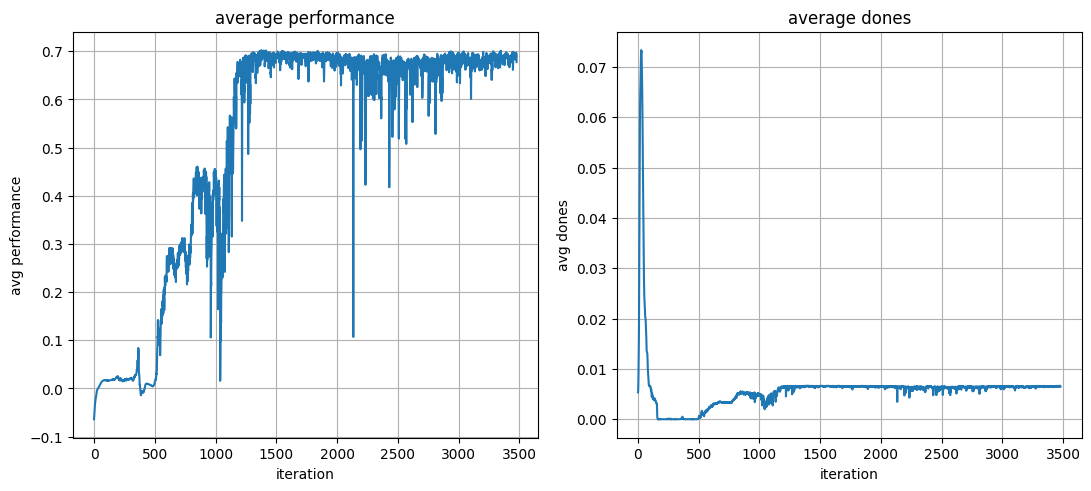
\includegraphics[width=\linewidth]{demo.png}
                \caption{The plot of the training progress.}
                \label{fig:training_progress}
            \end{figure}
            
    \end{itemize}

    The policy was trained upto 3400 iterations and I stopped it there because the curriculumFactor\_ is already closed to 1, so the performance should already be saturated.
    
\section{Future works}
There are a lot of rooms for the improvement from my work.
\begin{itemize}
    \item The training is not really reproducable. Therefore, I cannot experiment on how the effects of hyperparamters on the training. Probably designing the reward more carefully would help.
    \item The robot motion is not smooth because I did not impose any reward to make it do so. 
            Therefore, I think this motion might only be possible in the simulation. I should add more reward function, 
            for example, the reward that encourage the torque/ joint angles and joint velocity to be smooth compare to the previous values.
\end{itemize}

\section{Acknowledgement and feedback}
    First of all, thanks to Professor Hwangbo to allow me to audit the class. 
I really enjoy the contents of the class even though, sometimes, it is kind of hard to follow.
I really appreciated your efforts and patient to answer all of my questions and even gave your own opinions.
Thanks for your inspirational works and insights toward AI, RL and robotics, especially the tips on RL training. 
I think this kind of information came from your own experiences, in which we cannot find else where.
This would definitely be beneficial to my research and my career later on.

    Also, thanks to all the TAs that graded and gave the feedback to my works.

    As I am an auditor in this class, I could not give the feedback to the class using the Academic System. Therefore, I will write some here. I have a few suggestions if it could help to improve your class.

    \begin{itemize}
        \item The lecture is a bit hard to follow because the contents are difficult by itself (Probably you should demand some prerequisite classes, for example, RL). 
                So I think posting the material/ reading assignment earlier would definitely be much more helpful to understand all the concepts. 
                I know this is the first time you prepared the material so it is understandable.
        \item I like the quizes that you asked in the lectures (in the slides with red color). It is kind of a good checkpoint to check for my own understanding. 
                However, I found that sometimes your quiz is not for checking but rather to encourage discussion.
                In this case, I found that most of the time I will fail to give my own opinion because I still cannot understand the concept well. Probably, you could have a regular quiz to check student's concept 
                and a short discussion toward the end of the class.
        \item It's probably do a quick review from the last class to remind the student about the concepts they studied.
        \item I found that the programming assignments and final project are a bit irrelevant. 
        
              For the first assignment, we were checked for the value and policy iterations concept (I like the second part of the assignment as it looks like an unseen problem).
              
              For the second assignment, we did tabular Q-learning and tried to update with the RL algorithm. 
              
              But for the term project, the main tasked I did was the reward function design. So the concepts that we learned in the first two assignments were not useful here.

        \item I found that openAI Spinning Up in Deep RL is a good resource/ preliminary to what you have taught in the class. It is probably an appropriate reading assignment
                \url{https://spinningup.openai.com/en/latest/index.html}

    \end{itemize}

\end{document}